\documentclass[xcolor=pdftext, table]{beamer}
\usepackage{amsmath, amssymb, amsfonts, latexsym, stmaryrd}
%\usepackage[latin1]{inputenc}
\usepackage[T1]{fontenc}
\usepackage[utf8]{inputenc}
\usepackage[english, spanish]{babel}
% Tabla de tres secciones
\usepackage[flushleft]{threeparttable}

% \toprule, \midrule, \bottomrule
\usepackage{booktabs}
% Tablas con ancho establecido por usuario
\usepackage{tabularx}

% Para diagramas de bloques entre otros
\usepackage{smartdiagram}
\usesmartdiagramlibrary{additions}

% Para vinculos a archivos externos
\usepackage{hyperref}

% tikz
\usepackage{tikz}
\usetikzlibrary{arrows.meta, positioning, shadows}

\usefonttheme{professionalfonts}
%\usetheme{Bergen}
%\usetheme{Hannover}
%\usetheme{Boadilla}
%\usetheme{Luebeck}
%\usetheme{Warsaw}
\usetheme{AnnArbor}

\setbeamercovered{transparent}


% Definicion de colores tabla cronograma
\definecolor{colorfa}{rgb}{0.3569,0.608,0.8353}
\definecolor{colorfb}{rgb}{0.4392,0.678,0.2784}
\definecolor{colorfc}{rgb}{1.0000,0.361,0.0000}
\definecolor{colorsem}{rgb}{0.1804,0.455,0.7098}
\definecolor{colorfd}{rgb}{0.9294,0.490,0.1922}
\definecolor{colorfe}{rgb}{0.2667,0.329,0.4157}

% Definicion comandos tabla cronograma
\newcommand{\fa}{\cellcolor{colorfa}}
\newcommand{\fb}{\cellcolor{colorfb}}
\newcommand{\fc}{\cellcolor{colorfc}}
\newcommand{\sem}{\cellcolor{colorsem}}
\newcommand{\fd}{\cellcolor{colorfd}}
\newcommand{\fe}{\cellcolor{colorfe}}

% Definicion de tipos de columnas tabla
\newcolumntype{C}[1]{>{\centering}m{#1}}
\newcolumntype{L}[1]{>{\raggedleft}m{#1}}
\newcolumntype{R}[1]{>{\raggedright}m{#1}}

\setbeamertemplate{footline}
{
	\leavevmode%
	\hbox{%
		\begin{beamercolorbox}[wd=.4\paperwidth,ht=2.25ex,dp=1ex,center]{author in head/foot}%
		\usebeamerfont{date in head/foot}\insertshortauthor
		\end{beamercolorbox}%
		\begin{beamercolorbox}[wd=.6\paperwidth,ht=2.25ex,dp=1ex,center]%
			{title in head/foot}%
			\usebeamerfont{title in head/foot}\insertshorttitle\hspace*{3em}
			\insertframenumber{} / \inserttotalframenumber\hspace*{1ex}
		\end{beamercolorbox}}%
	\vskip0pt%
}

\setbeamertemplate{note page}[plain]

\begin{document}
	\title{Seminario Trabajo Especial de Grado}
	
	\subtitle{\large DISEÑO DE UN EQUIPO ELECTRÓNICO CONTROLADOR DE
		INTERRUPTORES Y ATENUADORES EMPLEADO EN LA
		MEDICIÓN DE LA FIGURA DE RUIDO EN DISPOSITIVOS DE
		RADIO FRECUENCIA}
		
	\author{{\bf Jose Arias}\\
		{Tutor: MSc. Pedro Ruiz}\\
		{Prof. Guía: Alejandro González}}		
		
	\institute{Universidad Central de Venezuela \\
		Facultad de Ingeniería \\
		Escuela de Ingeniería Eléctrica \\
		Departamento de Electrónica, Computación y Control}
	
	\date{Octubre 2017}
	
	%\logo{\includegraphics[height=1.5cm]{Imagenes/pie-der.pdf}}

	\frame{\titlepage}
	
	\section{Planteamiento del Problema}
	
	\begin{frame}
		\frametitle{Sistema para medición de figura de ruido (SMFR)}
	
		\begin{figure}[!h]
			\begin{center}
				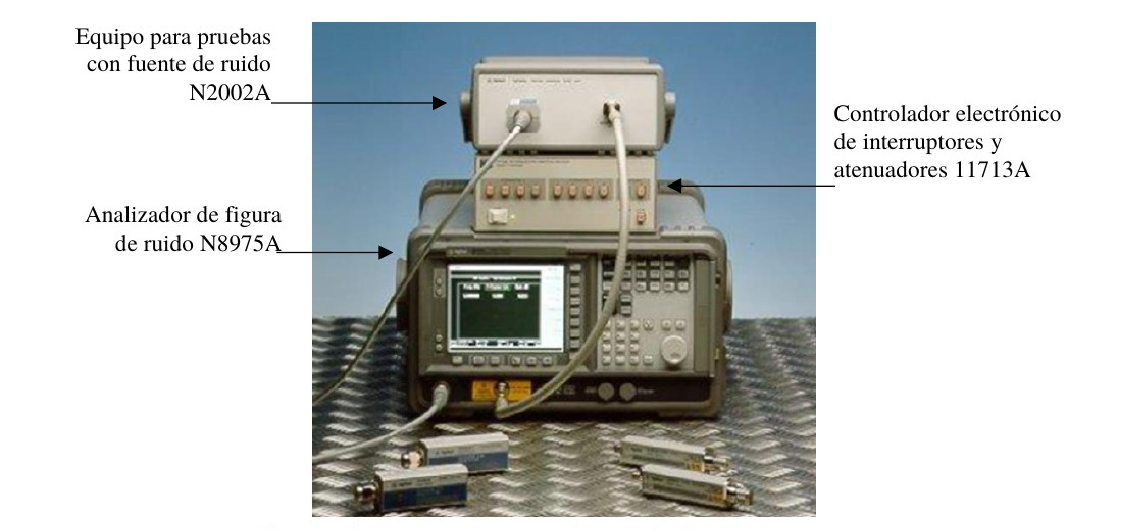
\includegraphics[height=6cm]{Imagenes/SistemaMedicionFiguraRuido.pdf}			
			\end{center}	
		\end{figure}
	
	\end{frame}


	\begin{frame}
		\frametitle{Dispositivos que integran el SMFR}
	
		\begin{table}[h!]
			\begin{tabular}{p{3cm}p{8cm}}
				\begin{minipage}{2cm}
					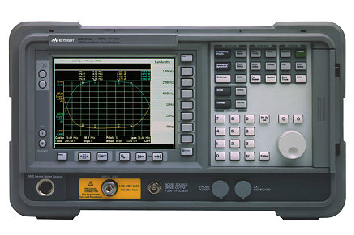
\includegraphics[width=3cm]{Imagenes/N8975A.pdf}
				\end{minipage} &
				Analizador de figura de ruido (NFA) N8975A \\
				
				\begin{minipage}{2cm}
					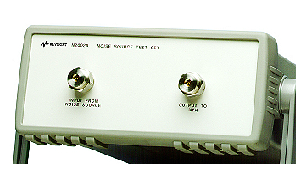
\includegraphics[width=3cm]{Imagenes/N2002A.pdf}
				\end{minipage} &
				Equipo para pruebas con fuente de ruido N2002A \\
				
				\begin{minipage}{2cm}
					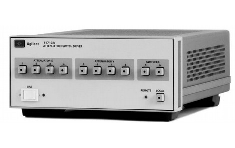
\includegraphics[width=3cm]{Imagenes/11713A.pdf}
				\end{minipage} &			
				Controlador electrónico de interruptores y atenuadores, serie 11713 
			\end{tabular}
		\end{table}		

	\end{frame}

	\begin{frame}
		\frametitle{Panorama del SMFR}			
	
		\begin{figure}
			\begin{center}
				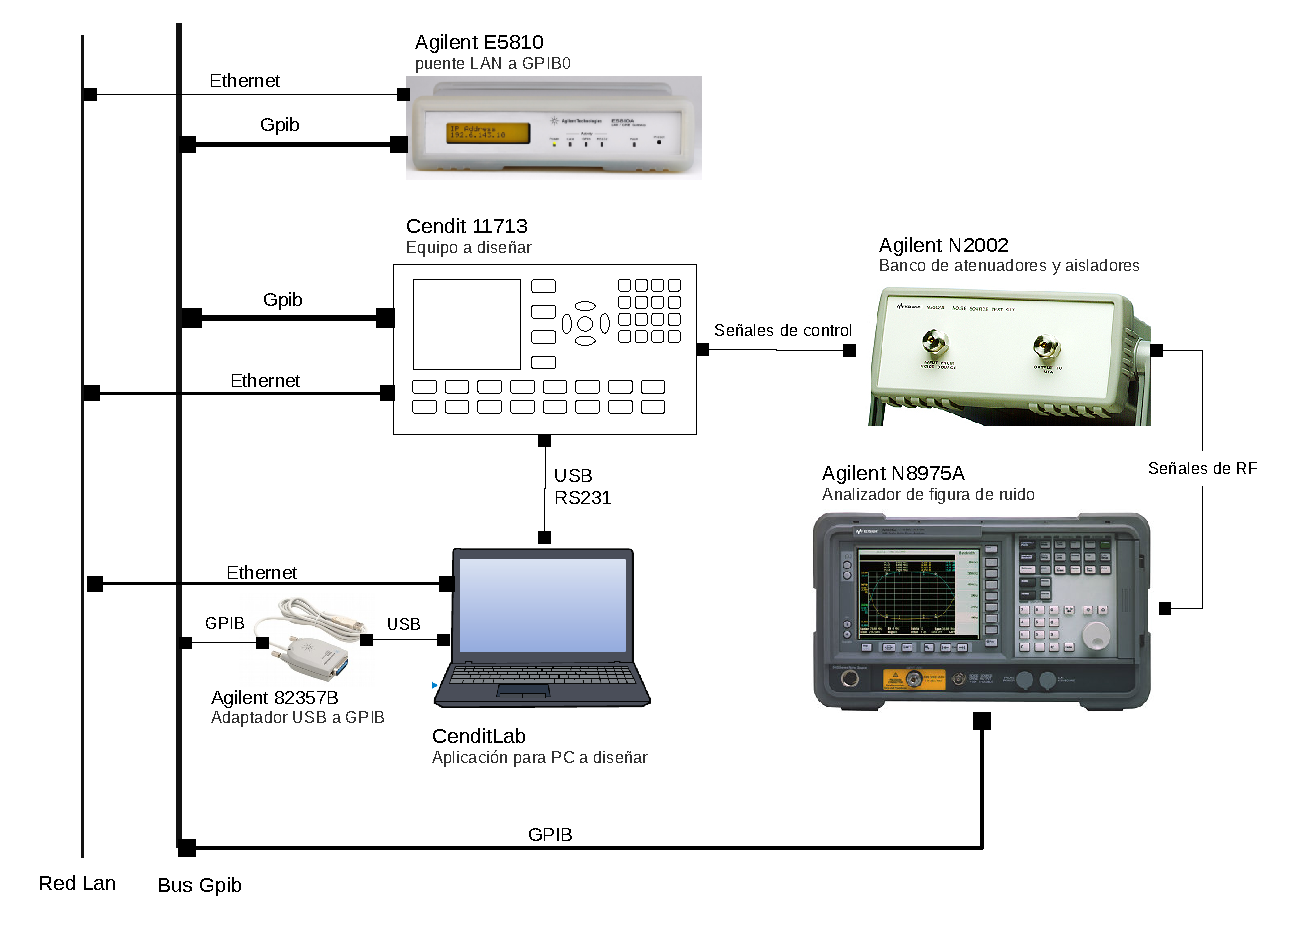
\includegraphics[width=10cm]{Imagenes/DiagramaBloquesSistema.pdf}
			\end{center}
		\end{figure}	
	
	\end{frame}

	\section{Metodología y Cronograma}
	
	\begin{frame}
		\frametitle{Metodología de trabajo}
	
		\begin{block}{Cronograma inicial}
			\begin{threeparttable}[!h]
				\centering
				\arrayrulecolor{gray}
				\setlength{\extrarowheight}{4pt}		
				\resizebox{\textwidth}{!}{
					\begin{tabular}{|c|l|l|l|l|l|l|l|l|l|l|l|l|l|l|l|l|l|l|l|l|l|l|l|l|l|l|l|l|}
						\hline 			
						\textbf{Semanas} & 1 & 2 & 3 & 4 & 5 & 6 & 7 & 8 & 9 & 10 & 11 & 12 & 13 & 14 & 15 & 16 & 17 & 18 & 19 & 20 & 21 & 22 & 23 & 24 & 25 & 26 & 27 & 28 \\
						\hline
						\textbf{Fase 1}
						& \fa & \fa & \fa & \fa & \fa & \fa & & & & & & & & & & & & & & & & & & & & & & \\			
						\hline			
						\textbf{Fase 2} & & & & & & & \fb & \fb & \fb & \fb & \fb & \fb & \fb & \fb & \fb & \fb & \fb & & & & & & & & & & & \\
						\hline
						\textbf{Fase 3} & & & & & & & & & & & & & & & & & & \fc & \fc & \fc & \fc & \fc & & & & & & \\	
						\hline		
						\textbf{Seminario} & & & & & & & & & & & & & & \sem & & & & & & & & & & & & & & \\
						\hline
						\textbf{Fase 4} & & & & & & & & & & & & & & & & & & & & & & & \fd & \fd & \fd & \fd &  & \\
						\hline
						\textbf{Fase 5} & & & & & & & & & & & & & & & & & & & & & & & & & & & \fe & \fe \\
						\hline	
					\end{tabular}
				}
				\begin{tablenotes}
					\item {\tiny Fecha de inicio: 6 de Marzo de 2017.} 
					\item {\tiny Jornada de 8 horas diarias, lunes a viernes, de 8:00 AM a 12:00 M y de 1:30 PM a 4:30 PM.}
				\end{tablenotes}
			\end{threeparttable}
		
			\begin{itemize}
				\item Fase 1: Preparación y documentación.
				\item Fase 2: Diseño de dispositivo.
				\item Fase 3: Implementación de dispositivo.
				\item Fase 4: Producción de manual de usuario. 
				\item Fase 5: Documentación TEG. 				
			\end{itemize}
		
		\end{block}

	\end{frame}

	\section{Tares Realizadas}
	
		\begin{frame}	
			\frametitle{División de tareas}

			\begin{block}{Organización en bloques del proyecto}		
				
			\begin{columns}			

				\begin{column}{8cm}			
					\begin{center}
						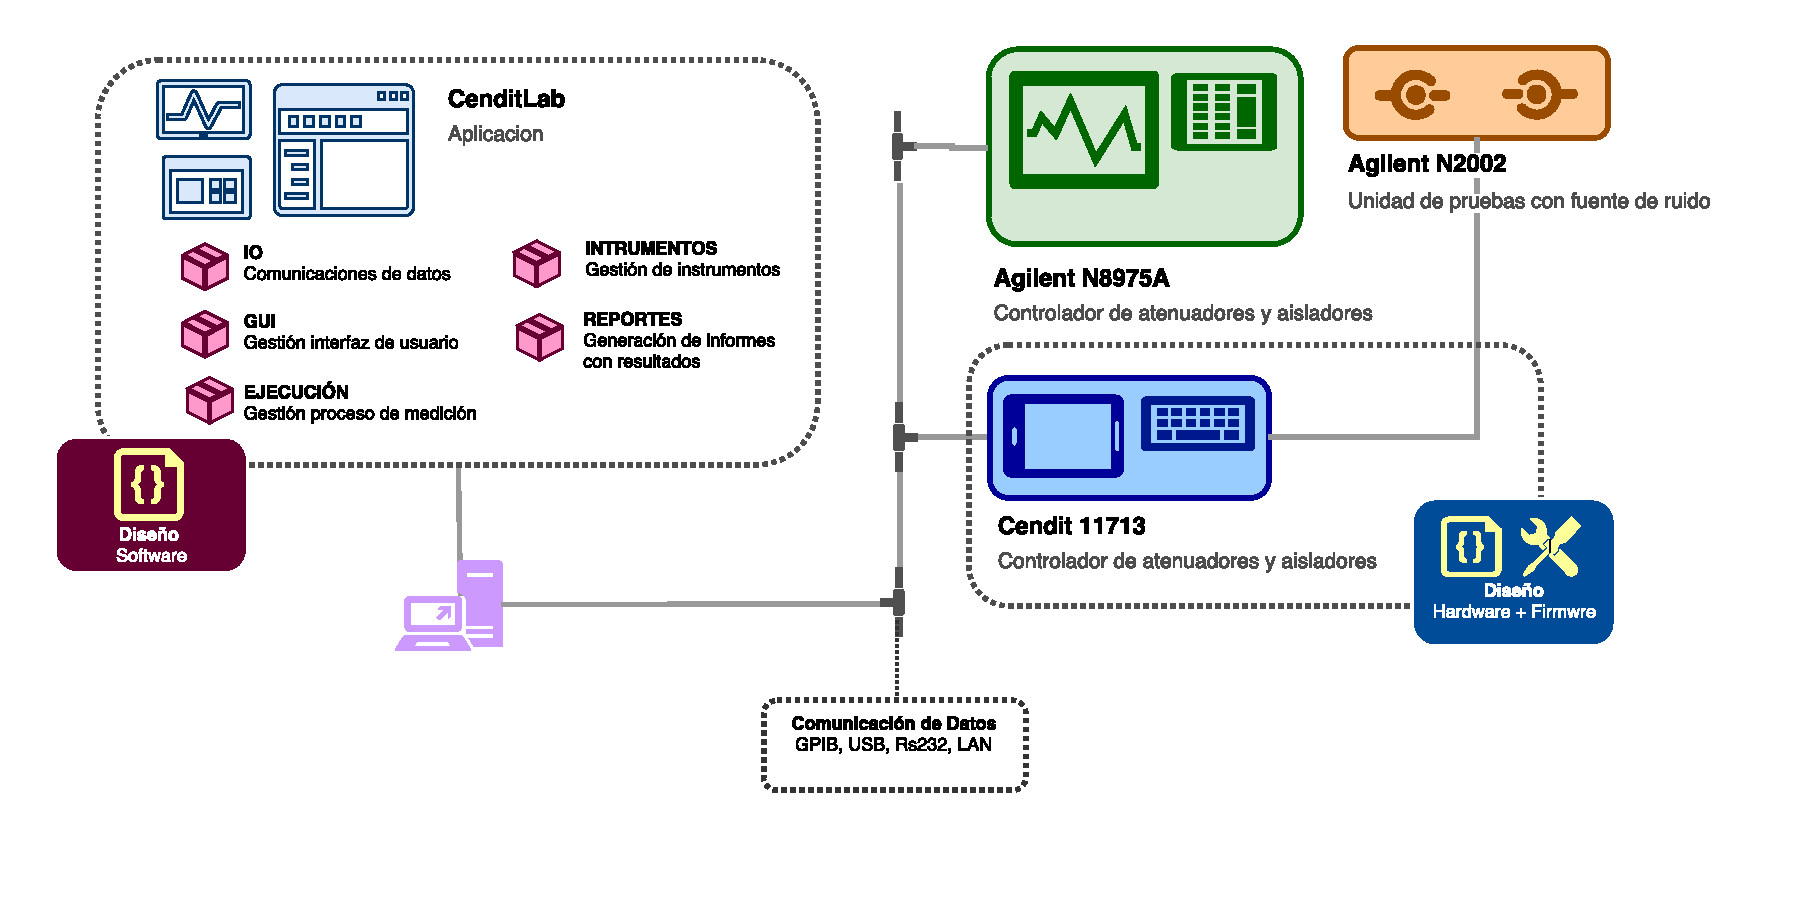
\includegraphics[width=8cm]{Imagenes/SystemMainDiagram.pdf}		
					\end{center}
				\end{column}
			
				\begin{column}{4cm}					
					\resizebox{4cm}{!}{
					\smartdiagram[constellation diagram]{Cendit 11713, 
						Hardware, Software, Firmware, Documentacion}}					
				\end{column}				
			\end{columns}
			
		\end{block}	
		
	\end{frame}

	\begin{frame}
		\frametitle{Documentación}
		
		\begin{itemize}
		 	\item Investigación sobre caracterización de dispositivos en alta frecuencia: parámetros de dispersión.
		 	\item Investigación sobre medición de figura de ruido en RF y microondas.
		 	\item Documentación acerca de cada uno de los instrumentos que integran el SMFR.
		 	\item Documentación acerca del software asociado o que brinda soporte al SMFR.				
		 \end{itemize}		

	\end{frame}

	\begin{frame}

	\frametitle{Software}
		\framesubtitle{Diseño de aplicación CenditLab}
		
		\begin{block}{Ciclo de diseño iterativo}			
			\centering
			\resizebox{6cm}{!}{
				\smartdiagramset{%
					circular distance=25mm,
					text width=20mm,
					module minimum width=30mm,
					module minimum height=10mm}
				
				\smartdiagram[circular diagram:clockwise]{Investigación, Modelado, Codificación, Pruebas}}		
		\end{block}	
	\end{frame}

	\begin{frame}
		\frametitle{Software}
		\framesubtitle{Diseño de aplicación CenditLab}		
		
		%\begin{columns}
		
		%	\begin{column}{7cm}
		\begin{block}{Diagrama de paquetes UML}
			\centering
			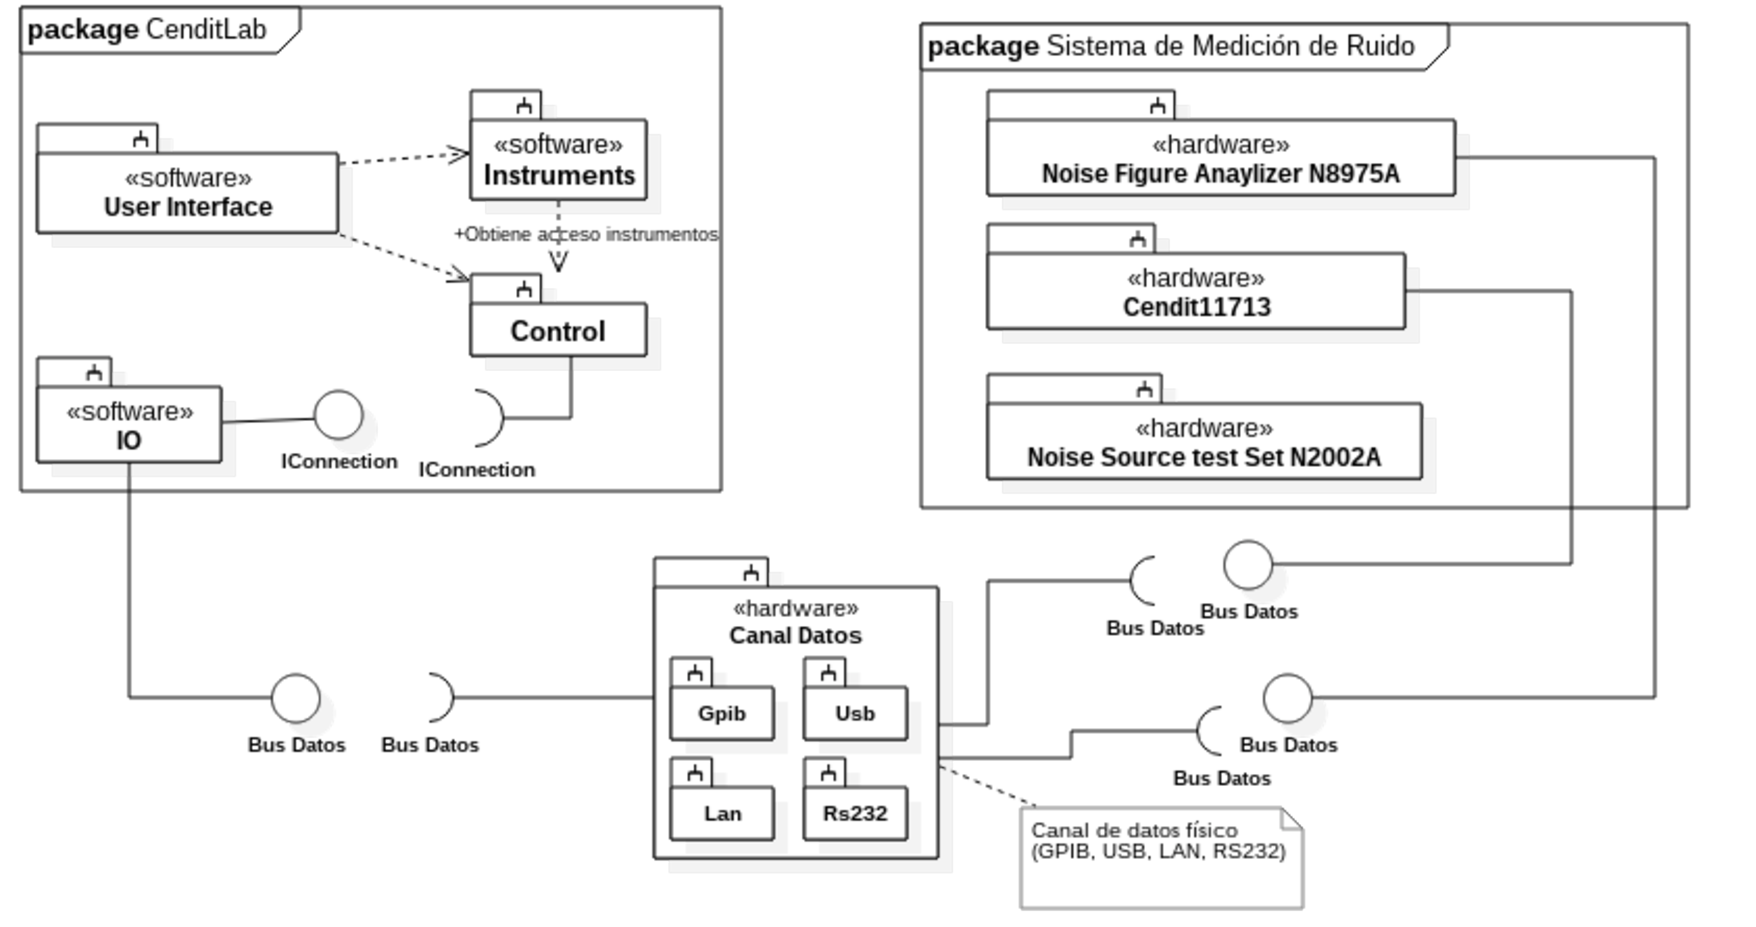
\includegraphics[width=7cm]{Imagenes/MainPackagesUml.pdf}
		\end{block}						
		%	\end{column}
		
		%	\begin{column}{5cm}				
		\begin{block}{Módulos de software principales}
			\begin{itemize}
				\tiny
				\item Interfaz de usuario
				\item Gestión de instrumentos
				\item Control del proceso de medición
				\item Gestión de comunicaciones
			\end{itemize}
		\end{block}
		%	\end{column}
		
		%\end{columns}	
	\end{frame}

	\begin{frame}
		\frametitle{Software}
		\framesubtitle{Ingeniería de software}
		
		\begin{block}{Captura de requerimientos}
			\begin{itemize}
				\item Estudio del software Test \& Measurement (T \& M) de Keysight Technologies (Keysight VEE Pro).
				\item Estudio de aplicaciones T \& M disponibles en el Cendit (EmcTest32).
				\item Entrevistas con personal técnico dentro del Cendit.
			\end{itemize}
		\end{block}	
		
		\begin{block}{Normas ISO/IEC/IEEE}
			\begin{itemize}  
				\small				
				\item Systems and Software Engineering: Architecture Description \\ {\footnotesize (ISO/IEC/IEEE 42010, 2011).}		
				\item System and Software Engineering: Life Cycle Processes Requirements Engineerng {\footnotesize (ISO/IEC/IEEE 29148, 2011).}
				\item Systems and Software Engineering: Vocabulary \\
				 {\footnotesize (ISO/IEC/IEEE 24765, 2011).}	
			\end{itemize}
		\end{block}
	
	\end{frame}

	\begin{frame} 
		\frametitle{Software}
		\framesubtitle{Requerimientos funcionales}


		\begin{block}{Requerimiento funcional 2}
			\begin{table}
				\tiny
				\begin{tabular}{rp{10cm}}	
					{ID:} & {FR2} \\
					{Título:} &  {Automatizar tareas de medición} \\
					{Descripción:} & {Los usuarios pueden programar los instrumentos y generar tareas de medición para sus posterior ejecución, de forma automatizada y remota} \\
					{Justificación:} & {Programar y automatizar las mediciones con el SMFR}\\
					{Dependencias:} & {FR1} \\
					{Usuario:} & {Técnico}	
				\end{tabular}
			\end{table}			
		\end{block}			
	
		\begin{block}{Requerimiento funcional 3}
			\begin{table}
				\tiny
				\begin{tabular}{rp{10cm}}	
					{ID:} & {FR3} \\
					{Título:} & {Presentar una interfaz gráfica para el SMFR} \\
					{Descripción:} & 	{La aplicación servirá como una representación integral en software de los tres instrumentos principales que componen el SMFR, será un instrumento virtual} \\
					{Justificación:} & {Simplificar las tares de medición con el SMFR} \\
					{Dependencias:} & {FR2} \\
					{Usuario:} & {Técnico} \\
				\end{tabular}
			\end{table}			
		\end{block}		
	
	\end{frame}

	\begin{frame} 
		\frametitle{Software}
		\framesubtitle{Requerimientos funcionales}	
		
		\begin{block}{Requerimiento funcional 4}
			\begin{table}
				\tiny
				\begin{tabular}{rp{10cm}}	
					{ID:} & {FR4} \\
					{Título:} & {Gestión de las comunicaciones con los instrumentos del SMFR de manera simple y uniforme desde la perspectiva de usuario} \\
					{Descripción:} & {La aplicación facilitará el intercambio de datos con los instrumentos del SMFR} \\
					{Justificación:} & {Simplificar la adquisición de datos del SMFR} \\
					{Dependencias:} & {FR1, FR2} \\
					{Usuario:} & {Técnico}	
				\end{tabular}
			\end{table}			
		\end{block}			
		

		\begin{block}{Requerimiento funcional 9}
			\begin{table}
				\tiny
				\begin{tabular}{rp{10cm}}	
					{ID:} & {FR9} \\
					{Título:} & {Capacidad para simular el proceso medición} \\
					{Descripción:} & {El usuario puede simular una tarea de instrumentación dada, sin necesidad de conexión con el SMFR} \\
					{Justificación:} & {Permitir al usuario ensayar una tarea de medición} \\
					{Dependencias:} & {FR2, FR3, FR4, FR5} \\
					{Usuario:} & {Técnico} \\
				\end{tabular}
			\end{table}			
		\end{block}		

	\end{frame}


	\begin{frame}
		\frametitle{Software}
		\framesubtitle{Recopilación e investigación de software asociado al SMFR}
		
		\begin{block}{Librerías oficiales}
			\begin{itemize}
				\item Virtual Instrument Software Architecture (VISA) \\
				{\small de National Instruments}
				\item IO Libraries Suite \\
				{\small de Keysight Technologies}
			\end{itemize}
		\end{block}
	
		\framebox[10cm]{Disponibles para Windows y ciertas distribucones de Linux}
		\framebox[10cm]{No disponibles en distribuciones Ubuntu ni Debian}	

	\end{frame}

	\begin{frame}
		\frametitle{Software}
		\framesubtitle{Desarrollo de librería alternativa para comunicación de datos}
		
		\begin{block}{Recopilación e investigación librerías alternativas}
			\begin{itemize}
				\item LinuxGPIB: acceso al bus GPIB.
				\item Vxi-11: acceso al bus GPIB a traves del un puente LAN/GPIB.
				\item Java Simple Serial Connector (jSSC): acceso al puerto RS-232 y USB CDC.
				\item libUsb: acceso al puerto USB.
			\end{itemize}
		\end{block}
		
	\end{frame}

	\begin{frame}	
		\frametitle{Software}
		\framesubtitle{Modelado y codificación de librería alternativa para comunicación de datos}
		
		\begin{columns}
			
			\begin{column}{5cm}
				\begin{block}{Módulo GPIB}
					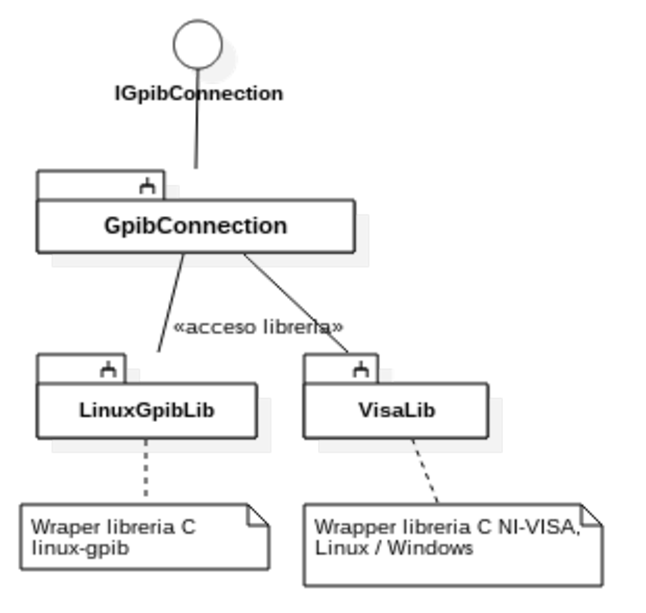
\includegraphics[width=5cm]{Imagenes/GpibConnectionPackageUml.pdf} 
				\end{block}			
			\end{column}
		
			\begin{column}{5cm}
				\begin{block}{Módulo Lan}
					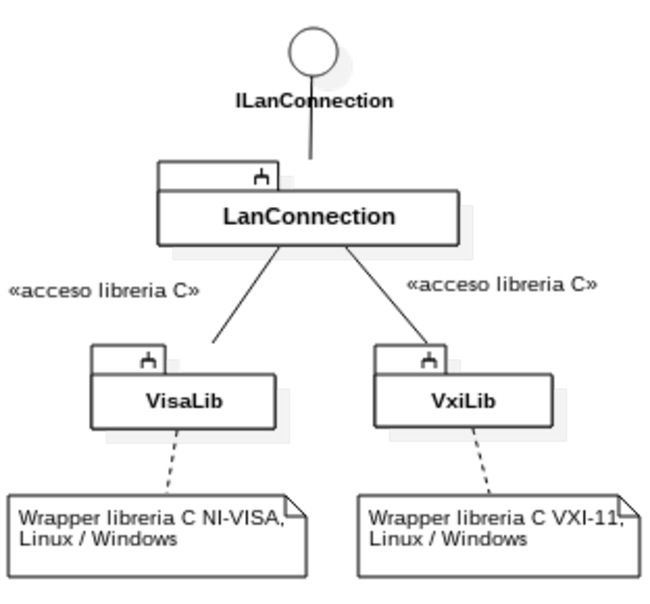
\includegraphics[width=5cm]{Imagenes/LanConnectionPackageUml.pdf}
				\end{block}				
			\end{column}	
				
		\end{columns}		
	
	\end{frame}

	\begin{frame}	
		\frametitle{Software}
		\framesubtitle{Modelado y codificación de librería alternativa para comunicación de datos}

		\begin{columns}
	
			\begin{column}{3cm}
				\begin{block}{Módulo Serial}
					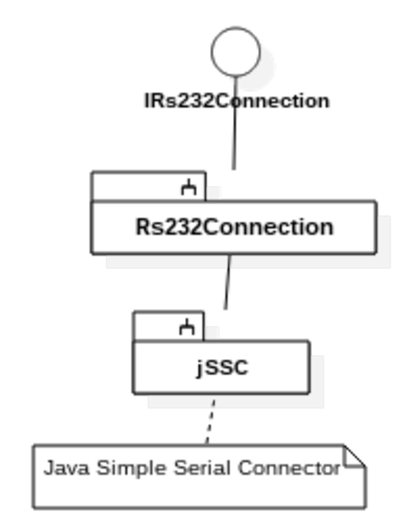
\includegraphics[width=3cm]{Imagenes/Rs232ConnectionPackageUml.pdf} 
				\end{block}			
			\end{column}
		
			\begin{column}{6cm}
				\begin{block}{Módulo USB}
					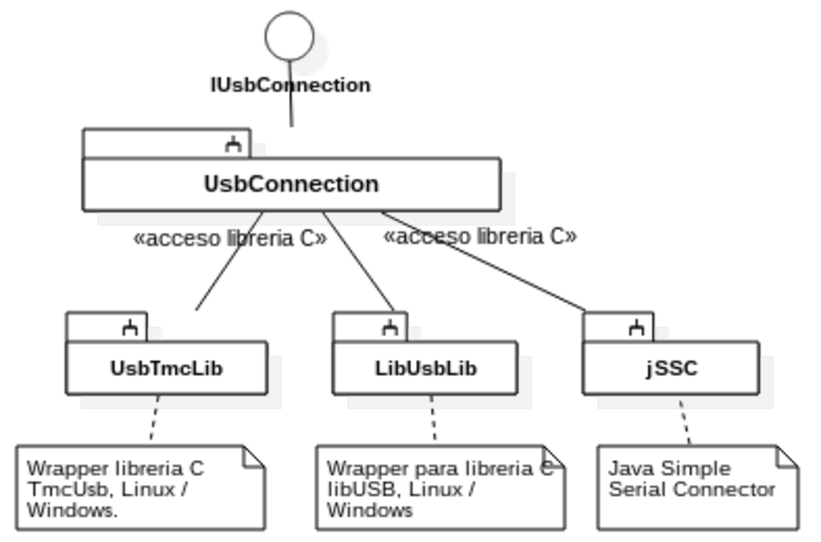
\includegraphics[width=6cm]{Imagenes/UsbConnectionPackageUml.pdf}	
				\end{block}				
			\end{column}	
	
		\end{columns}

	\end{frame}

	\begin{frame}	
		\frametitle{Software}
		\framesubtitle{Modelado y codificación de librería alternativa para comunicación de datos}

		\begin{block}{Diagrama de paquetes UML}
			\centering
			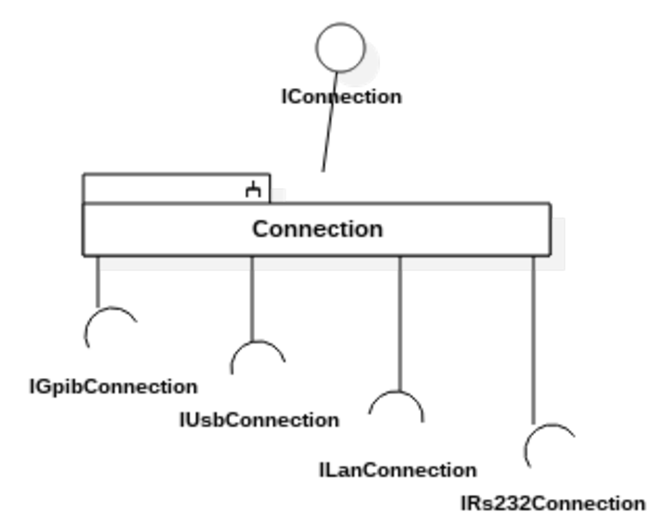
\includegraphics[width=7cm]{Imagenes/ConnectionPackageUml.pdf}
		\end{block}

	\end{frame}

	\begin{frame}
		\frametitle{Hardware}
		\framesubtitle{Estudio comparativo de los dispositivos de la serie 11713}
		
		\begin{block}{Vistas del panel frontal}
			\begin{table}
				\resizebox{10cm}{!}{
				\centering
				\begin{tabular}{ccc} 		
					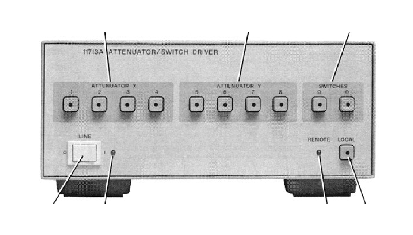
\includegraphics[width=5cm]{Imagenes/front-11713A.pdf} &
					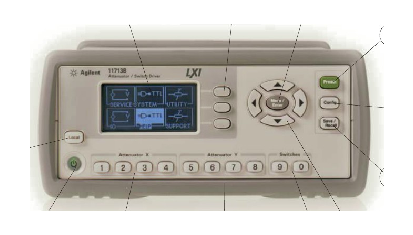
\includegraphics[width=5cm]{Imagenes/front-11713B.pdf} &
					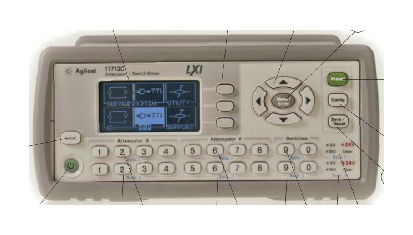
\includegraphics[width=5cm]{Imagenes/front-11713C.pdf} \\			
					Agilent 11713A & Keysight 11713B & Keysight 11713C \\
				\end{tabular}}
			\end{table}
		\end{block}
		
		\begin{block}{Vistas del panel posterior}
			\begin{table}
				\resizebox{10cm}{!}{
				\centering
				\begin{tabular}{ccc} 		
					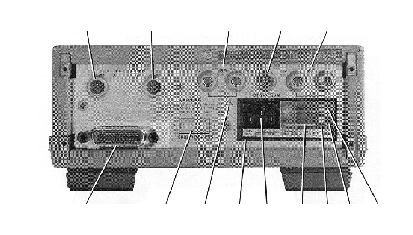
\includegraphics[width=5cm]{Imagenes/back-11713A.pdf} &
					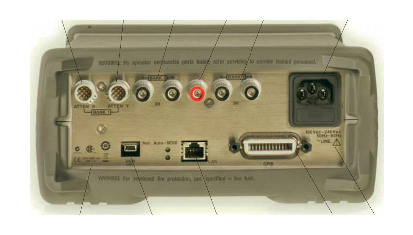
\includegraphics[width=5cm]{Imagenes/back-11713B.pdf} &
					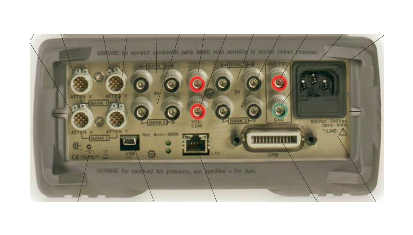
\includegraphics[width=5cm]{Imagenes/back-11713C.pdf} \\			
					Agilent 11713A & Keysight 11713B & Keysight 11713C \\
				\end{tabular}}
			\end{table}
		\end{block}		
	
	\end{frame}

	\begin{frame}
		\frametitle{Hardware}
		\framesubtitle{Identificación de características clave}
		
		\begin{columns}
			
			\begin{column}{6cm}
				
				\begin{block}{Características eléctricas}					
					\begin{itemize}
						\tiny
						\item Soporte para 2 puertos Viking.
						\item Soporte para dos jack banana.
						\item Suministro de alimentación DC programable.
					\end{itemize}
				\end{block}		
			
				\begin{block}{Interfaz de usuario}				
					\begin{itemize}
						\tiny
						\item Pantalla LCD.
						\item Teclado alfanumérico.
					\end{itemize}
				\end{block}			
			
			\begin{block}{Interfaces de comunicaciones}
				\begin{itemize}
					\tiny
					\item USB
					\item LAN
					\item GPIB
				\end{itemize}
			\end{block}							

			\end{column}
		
			\begin{column}{4cm}
				
				\begin{block}{\small Keysight 11713B}
					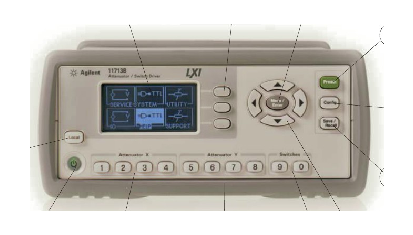
\includegraphics[width=4cm]{Imagenes/front-11713B.pdf} \\
					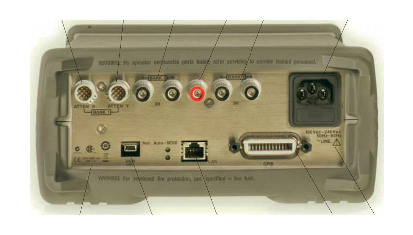
\includegraphics[width=4cm]{Imagenes/back-11713B.pdf}
				\end{block}
											
			\end{column}		
		
		\end{columns}
	
	\end{frame}

	\begin{frame}
		\frametitle{Hardware}
		\framesubtitle{Elaboración de concepto de diseño}
		
		%\begin{figure}[h!]
		%	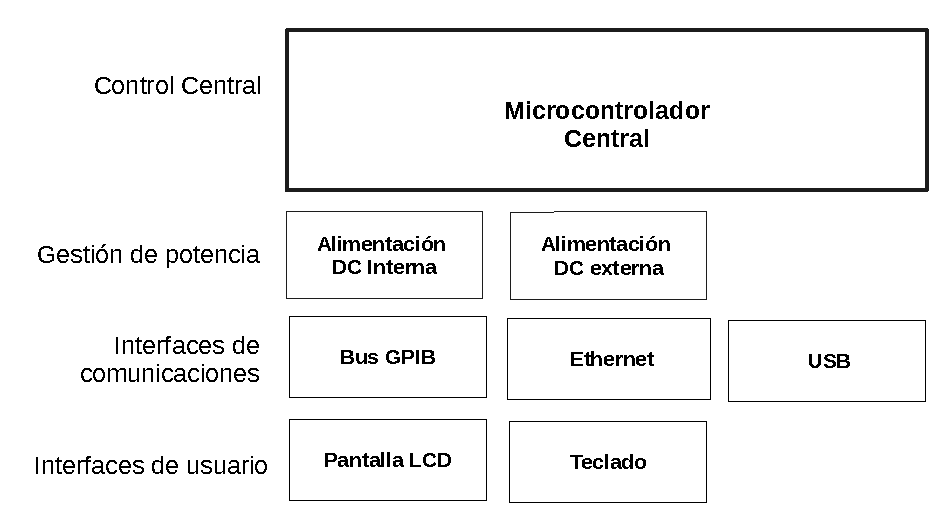
\includegraphics[width=6cm]{Imagenes/EsquemaConceptualCendit11713.pdf}		
		%	\caption{Esquema conceptual para el sistema Cendit11713.}
		%	\label{Fig:EsquemaConceptualCendit11713}
		%\end{figure}		
	
		\begin{figure}[h!]
			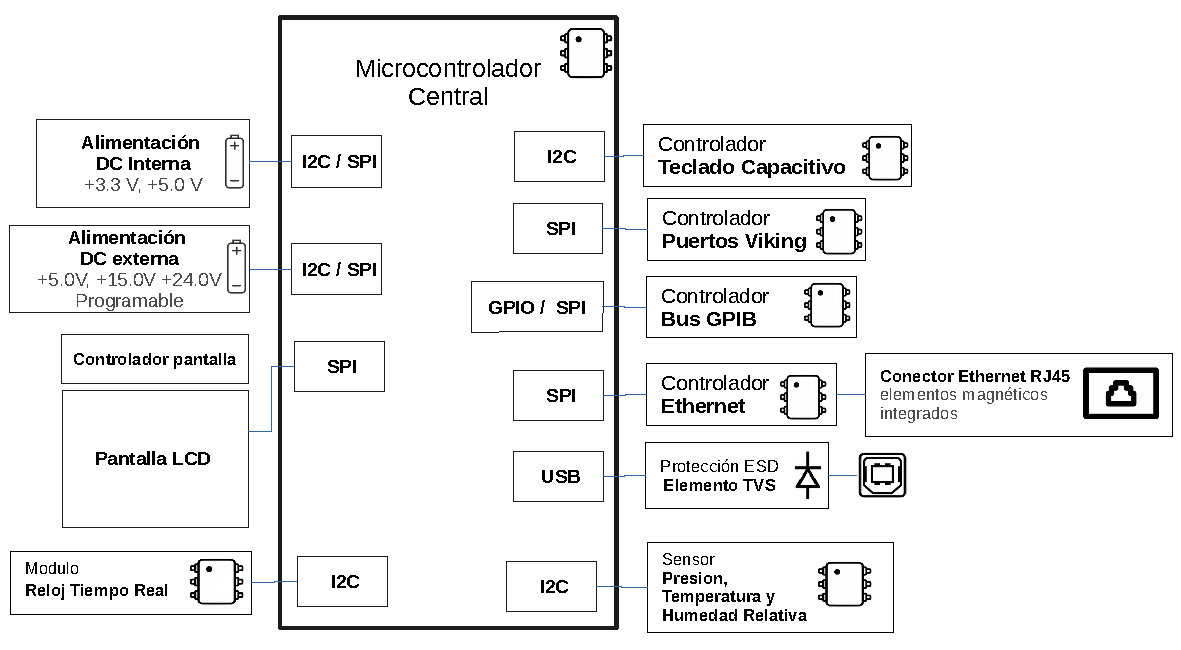
\includegraphics[width=10cm]{Imagenes/EsquemaCendit11713Detallado.pdf}		
		\end{figure}
	
	\end{frame}

	\begin{frame}
		\frametitle{Hardware}
		\framesubtitle{Diseño módular de tarjetas PCB}
		
		\begin{figure}[h!]
			\centering
			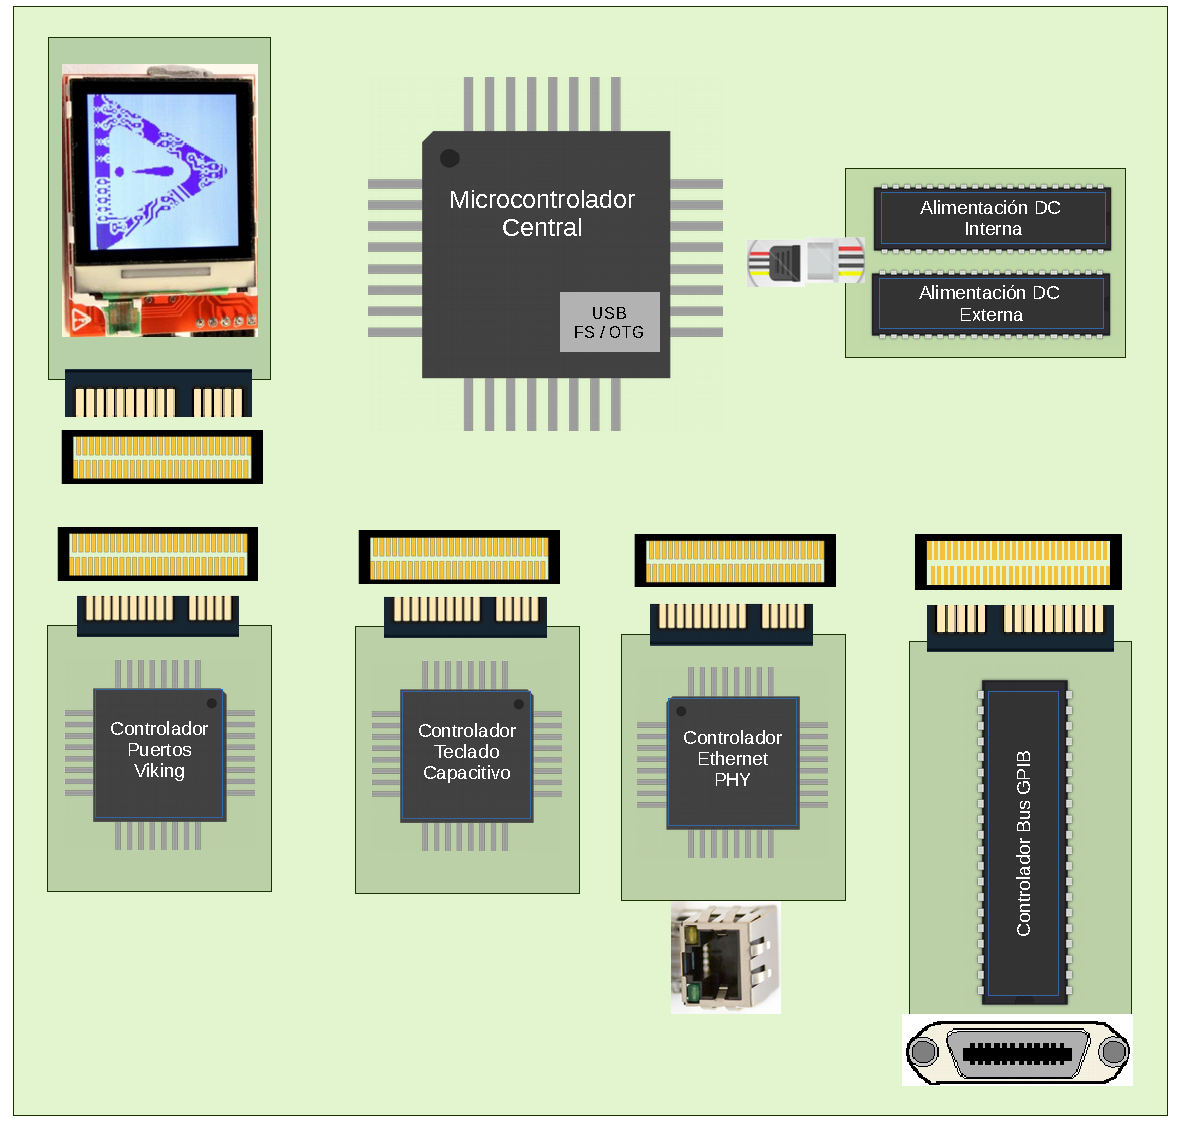
\includegraphics[width=7cm]{Imagenes/EsquemaCircuitoImpresoCendit11713_2.pdf}
		\end{figure}
	\end{frame}

	\begin{frame}  
		\frametitle{Hardware}
		\framesubtitle{Selección de componentes. Circuitos integrados}
		
		\begin{block}{Selección de microcontrolador de 32 bits}
			\centering
			\resizebox{\textwidth}{!}{
				\begin{tabular}{cC{3cm}ccccc}
					\toprule
					MCU & Descripción & Flash (kB) & SRAM (kB) & Encapsulado & USB & Ethernet \\
					\midrule
					TM4C129ENCPDT & ARM Cortex-M4F 120 MHz & 1024 & 256 & TQFP-128 & H/D/OTG & MAC-PHY \\
					LPC1768FBD1 & ARM Cortex-M3 100 MHz& 512 & 64 & LQFP-100 & D/H/OTG & MAC \\
					MKL26Z256VLL4 & Kinetis KL26 Cortex-M0+ 48 MHz & 256 & 32 & LQFP-100 & FS & NO \\
					\bottomrule
				\end{tabular}
			}		
		\end{block}
		
		\begin{block}{Selección de microcontrolador de 8 bits}
			\centering	
			\resizebox{\textwidth}{!}{
				\begin{tabular}{cC{3cm}ccccc}
					\toprule
					MCU & Descripción & Flash (kB) & SRAM (kB) & Encapsulado & USB & Ethernet \\
					\midrule
					PIC18F4550 &  MCU PIC18 8 bits & 32 & 2 & DIP-40 & D & NO \\
					PIC1845K50 & MCU PIC18 8 bits & 32 & 2 & TQFP-44 & D & NO \\
					PIC18F67J60 & MCU PIC18 8 bits& 128 & 3.8 & TQFP-64 & NO & 10/100/1000 Base-T \\
					\bottomrule
				\end{tabular}}		
		\end{block}
		
	\end{frame}

	\begin{frame}  
		\frametitle{Hardware}
		\framesubtitle{Selección de componentes. Circuitos integrados}
		
		\begin{block}{Selección para controlador de teclado}			
			\centering
			\resizebox{\textwidth}{!}{
				\begin{tabular}{cC{3cm}ccc}
					\toprule
					Parte & Descripción & Encapsulado & Comunicaciones & Fabricante\\
					\midrule
					PCF8885 & Controlador de teclado capacitivo de 8 canales & TSSOP-28 & I2C (FM+) & NXP  \\
					\bottomrule
				\end{tabular}
			}		
		\end{block}
		
		\begin{block}{Selección para expansor de puertos Viking}					
			\centering
			\resizebox{\textwidth}{!}{
				\begin{tabular}{cC{3cm}ccc}
					\toprule
					Parte & Descripción & Encapsulado & Comunicaciones & Fabricante\\
					\midrule
					MC33996 & Interruptor de 16 salidas & SOIC-32 & SPI & NXP  \\
					\bottomrule
				\end{tabular}
			}		
		\end{block}	
	
	\end{frame}

	\begin{frame}
		\frametitle{Hardware}
		\framesubtitle{Selección de componentes. Circuitos integrados}
		
		\begin{block}{Selección para controlador de Ethernet}		
			\centering
			\resizebox{\textwidth}{!}{
				\begin{tabular}{cC{5cm}cC{4cm}c}
					\toprule
					Parte & Descripción & Encapsulado & Comunicaciones & Fabricante\\
					\midrule
					ENC28J60 & Controlador Ethernet 10/100/1000Base-T MAC con 10Base-T PHY & SOIC-28 & SPI & Microchip  \\
					CP2200 &  Controlador Ethernet 100/1000 Base-T 10 Base-T PHY & TQFP-48 & Bus paralelo Intel o Motorola & Silicon Labs \\
					CP2201 &  Controlador Ethernet 100/1000 Base-T 10 Base-T PHY & QFN-28 & 
					Bus paralelo Intel o Motorola multiplexado & Silicon Labs \\				
					\bottomrule
				\end{tabular}
			}		
		\end{block}
	
		\begin{block}{Selección para transceptores de bus GPIB}
			\centering		
			\resizebox{10cm}{!}{				
				\begin{tabular}{cC{4cm}cc}
					\toprule
					Parte & Descripción & Encapsulado & Fabricante\\
					\midrule
					SN75ALS160 & Transceptor de bus octal IEEE 488 (bus datos) & SOIC-20 & Texas Instruments \\
					SN75ALS162 & Transceptor de bus octal IEEE 488 (bus control) & SOIC-20 & Texas Instruments \\
					\bottomrule
				\end{tabular}
			}		
		\end{block}	
		
	\end{frame}

	\begin{frame}
		\frametitle{Hardware}	
		\framesubtitle{Selección de componentes. Circuitos integrados}
		
		\begin{block}{Selección de IC para control de alimentación DC}	
			\centering
			\resizebox{\textwidth}{!}{
			\begin{tabular}{cC{4cm}cc}
				\toprule
				Parte & Descripción & Encapsulado & Fabricante\\
				\midrule
				XR77129 & PMIC, controlador reductor cuadruple PWM/PFM 40V programable &
				QFN-44 & Exar Corporation \\
				XR77103 & PMIC reductor de 3 salidas programables 14V & TQFN-32 & Exar Corporation \\				
				XR79110 & Módulo de potencia COT reductor síncrono de 22V 10A & QFN-72 & Exar Corporation \\
				TL494 & Controlador de ancho de pulso & SOIC-16 / PDIP-16 & Texas Instruments \\
				\bottomrule
			\end{tabular}}
		\end{block}				
	\end{frame}

	\begin{frame}
		\frametitle{Hardware}	
		\framesubtitle{Diseño de circuitos impresos}
		
		\begin{block}{Elaboración de esquemáticos}
			\begin{itemize}
				\item \href{run:./Documentos/MainBoardSchematic.pdf}{Tarjeta principal basada en microcontrolador PIC18F45K50}
				\item \href{run:./Documentos/PortExpanderMC33996.pdf}%
					{Expansor de puertos Viking basado IC MC33996}
				\item \href{run:./Documentos/CapacitiveKeyboardPCF8885.pdf}%
					{Controlador de teclado capacitivo basado en IC PCF8885}
				\item Tarjeta para pruebas pantalla LCD Nokia 1600
			\end{itemize}
		\end{block}		
		
	\end{frame}

	\begin{frame}
		\frametitle{Tareas pendientes}	
			
			\begin{block}{Software}
				Culminar el diseño de la aplicación CenditLab
				\begin{itemize}
					\item Librerías de soporte de comunicaciones IO para Windows
					\item Culminar módulo gestión GUI
					\item Culminar módulos de gestión de instrumentos
					\item Culminar módulos de gestión de medición
				\end{itemize}
					
			\end{block}		

		\end{frame}
	
	\begin{frame}
	
	\frametitle{Tareas pendientes}		
	
		\begin{block}{Firmware}
			Iniciar el diseño y generación de firmware Cendit 11713
			\begin{itemize}
				\item Control de expansor de puertos Viking
				\item Comunicaciones por medio del bus USB
				\item Comunicaciones a través de redes LAN (TCP/IP)
				\item Gestión de la fuente de alimentación
				\item Gestión de la interfaz de usuario (teclado y pantalla)
			\end{itemize}
		\end{block}

	\end{frame}	

	\begin{frame}
		\frametitle{Tareas pendientes}			
	
		\begin{block}{Hardware}
			Culminar diseños, construcción y depuración para los módulos 
			\begin{itemize}
				\item Fuente de alimentación
				\item Teclado capacitivo
				\item Expansor de puertos Viking 
				\item Módulo Ethernet
				\item Pantalla LCD	
				\item Tarjeta madre				
			\end{itemize}
		\end{block}
	
	\end{frame}
\end{document}